\chapter{Week 3: Python op de Pi}

Nu we enige basis van \textit{Python} bezitten, en wat ervaring hebben met de taal in combinatie op je laptop/pc, gaan we deze week aan de slag met de \textit{Raspberry Pi}. We gaan er deze week voor zorgen dat je je een beetje wegwijs maakt op dit kleine machientje, en dan gaan we aan de slag met de \textit{GPIO}-poorten van de \textit{Pi} in \textit{Python}. Maar voordat we dat doen, gaan we eerst kijken naar een ander belangrijk concept: \textit{loops}. 

\section{Loops}\index{Loops}
Als we bepaalde onderdelen van onze code vaker uit willen voeren, kunnen we dat doen aan de hand van \textit{loops}. In \textit{C} hadden we al kennisgemaakt met de \pyth{for}-loop. Deze zit gelukkig ook in \textit{Python}, maar werkt wel een beetje anders. We gebruiken deze vaak in combinatie met de funtie \pyth{range()}:
\begin{python}
for x in range(0, 10, 1):
	print(x)
\end{python}
In het bovenstaande voorbeeld roepen we de functie \pyth{range()} aan met 3 argumenten($0$, $10$ en $1$). De eerste geeft het startgetal voor $x$ aan, de tweede bij welke waarde van $x$ de loop moet stoppen, en de derde en laatste met welke hoeveel we $x$ we moeten verhogen bij elke nieuwe iteratie. Dit voorbeeld print dus de getallen $0$ t/m $9$ op het scherm:
\begin{python}
0
1
2
3
4
5
6
7
8
9
\end{python}

\begin{remark}
De functie \pyth{range()} kun je op $3$ verschillende manieren aanroepen:
\begin{enumerate}
\item[-] \pyth{range(stop)}: Met enkel $1$ argument, de stop waarde. $start=0, step=1$.
\item[-] \pyth{range(start, stop)}: Met $2$ argumenten, voor start en stop. $step=1$.
\item[-] \pyth{range(start, stop, stap)}: En $3$, zoals in het voorbeeld.
\end{enumerate}
In het bovenstaande stukje voorbeeldcode kan dus \pyth{range(0, 10, 1)} worden vervangen door \pyth{range(10)}, want die levert dezelfde functionaliteit.
\end{remark}

Als tweede voorbeeld een loop die van $2$ t/m $25$ loopt, met stapjes van $3$:
\begin{python}
for x in range(2, 25, 3):
	print(x)
\end{python}
Dit print het volgende uit: $2, 5, 8, 11, 14, 17, 20, 23$. De \pyth{for}-loop stopt na $23$, omdat $23+3 = 26$, wat hoger is dan $25$, de stop waarde. \newline

Naast de \pyth{for}-loop, bestaat er ook de \pyth{while}-loop. Deze zit ook in \textit{C}, maar hebben we destijds niet gebruikt. Wellicht is het handig om te weten dat hij bestaat, en te snappen hoe je 'm gebruikt:
\begin{python}
i = 1
while i < 6:
	print(i)
	i += 1
\end{python}
In het bovenstaand voorbeeld wordt de code in de \pyth{while}-loop uitgevoerd \textit{zolang} de conditie \pyth{i < 6} gelijk is aan \pyth{True}. We beginnen met \pyth{i = 1}, en tellen er elke keer \pyth{1} bij op, waardoor de uitvoer van het programma $1$ t/m $5$ is. \newline

Met een \pyth{while}-loop is ook vrij makkelijk een oneindige loop te maken, vergelijkbaar met de \textit{loop()}-functie bij de \textit{Arduino}:
\begin{python}
while True:
	print('en door..')
\end{python}

\begin{remark}
Het is bij zo'n loop wel handig om te weten hoe je 'm weer stopt. Want in de meeste gevallen maak je 'm per ongeluk. Bij een \textit{IDE} heb je naast een run knopt (groen driehoekje), vaak ook een stop knop (rood vierkantje). In de terminal kun je de toetscombinatie \text{Ctrl+C} gebruiken. 
\end{remark}

\newpage

\section{Editor}\index{Editor}
Nu het concept van loops ook bekend is in \textit{Python} gaan we ons richtin op de \textit{Raspberry Pi}. Allereerst, is net als bij je laptop ook op de \textit{Pi} handiger om een \textit{IDE} te gebruiken. Dus daar gaan we eerst voor zorgen. Als het goed is staat \textit{Thonny} standaard geïnstalleerd, maar ook hier mag je alles gebruiken wat je zelf prettig vindt. Tijdens de lessen wordt zoals eerder vermeld met Thonny gewerkt. \newline

Mocht \textit{Thonny} of je favoriete editor nog niet geïnstalleerd zijn, is dit een mooi moment om te kijken dat eigenlijk gaat onder \textit{Linux}. Je kunt hiervoor de grafische \textit{Add/Remove Software}-tool voor gebruiken:
\begin{figure}[h!]
\centering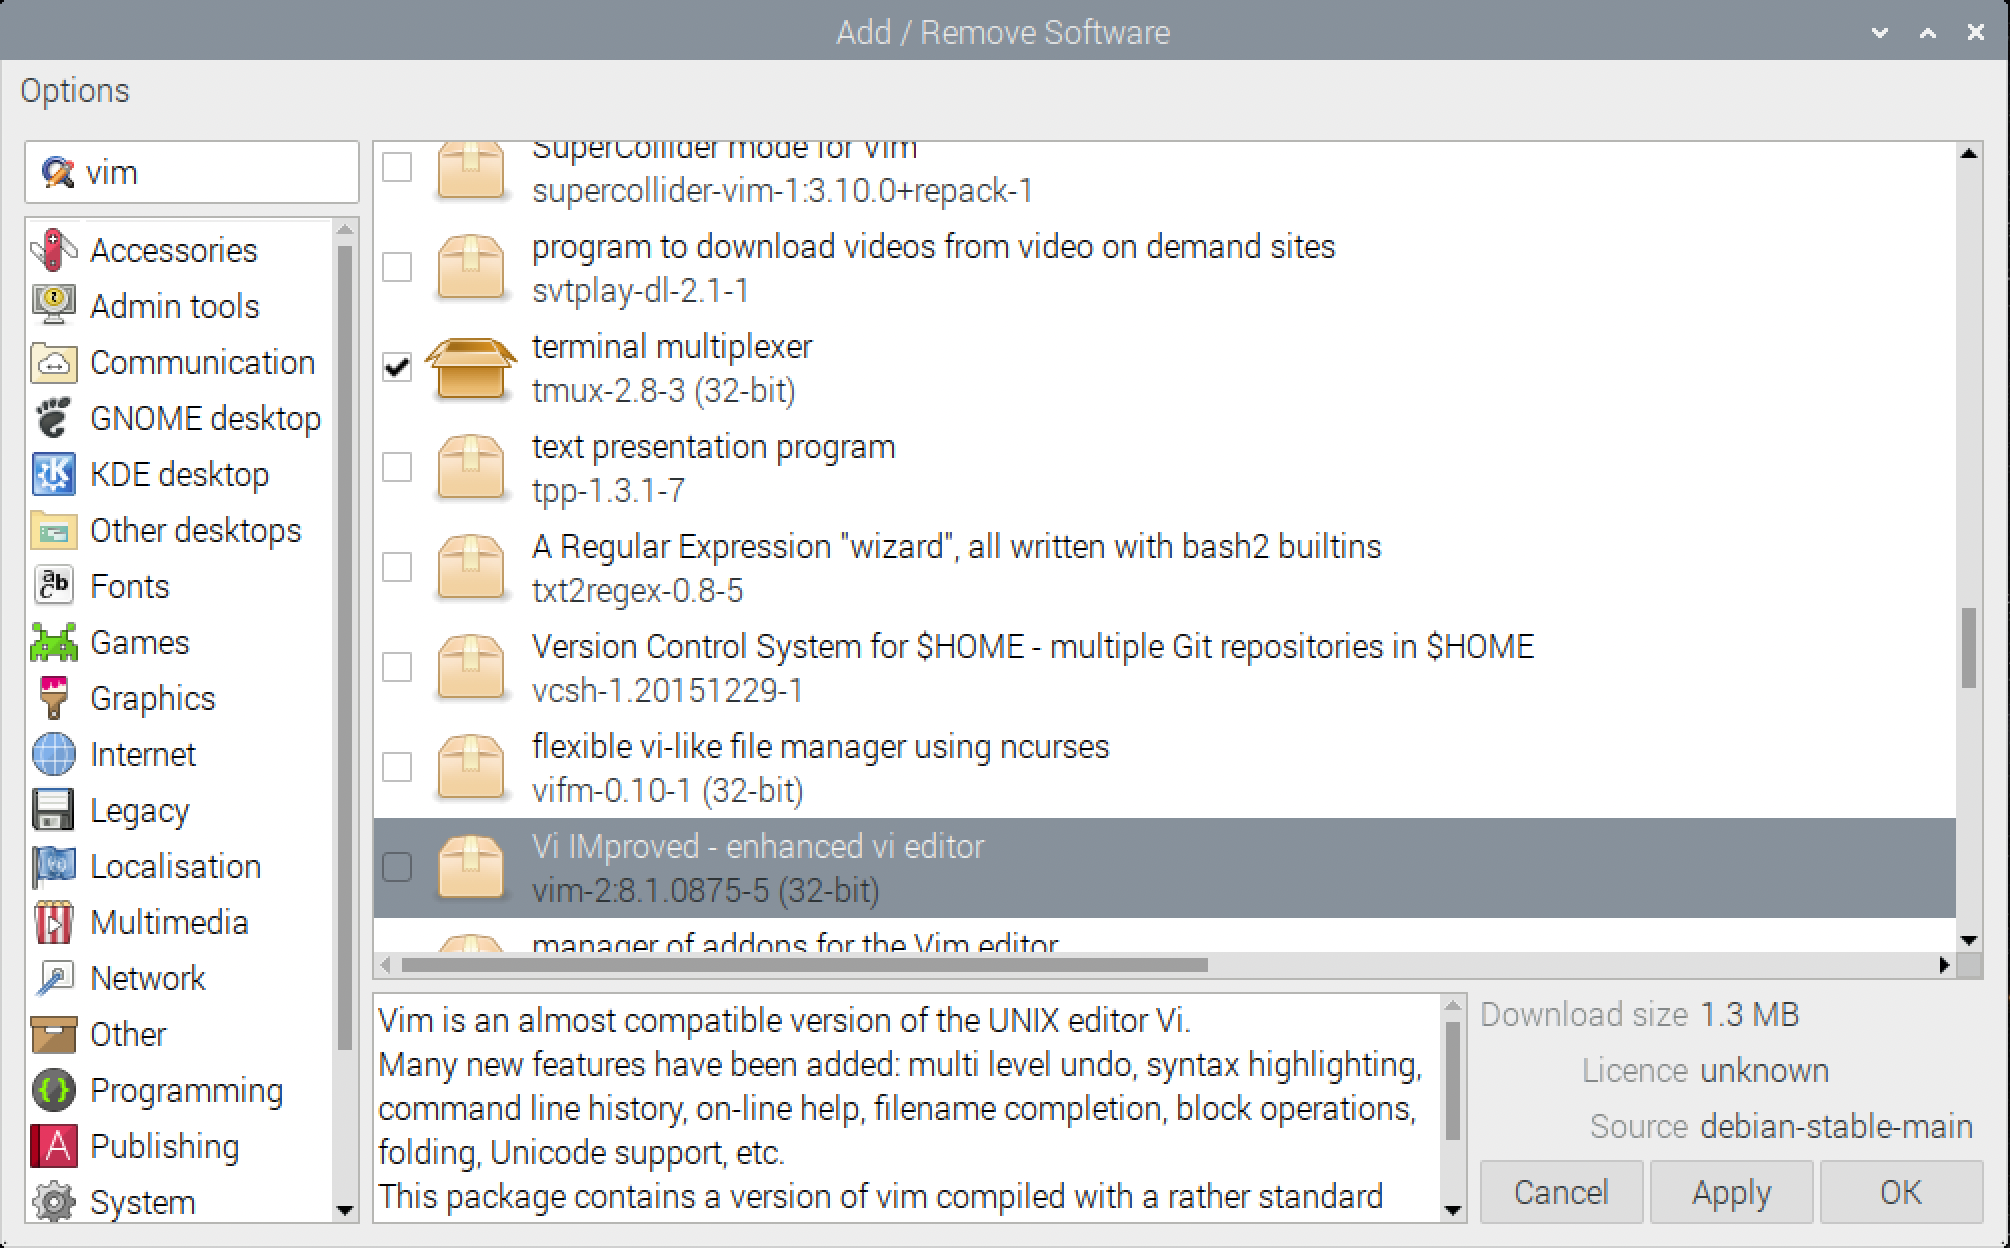
\includegraphics[scale=0.25]{Pictures/chapter05/add_remove_software.png}
\caption{\textit{Add/Remove Software} tool}
\label{fig:addremovesoftware} % Unique label used for referencing the figure in-text
%\addcontentsline{toc}{figure}{Figure \ref{fig:webserver}} % Uncomment to add the figure to the table of contents
\end{figure}

\begin{remark}
Een beetje hacker doet dit vaak via de \textit{Terminal}. Ook omdat de \textit{Pi} niet altijd aangesloten is op een scherm, is het ook handig om te weten hoe dit werkt. Allereerst zorg je ervoor dat alle lijsten met software die je kunt installeren up-to-date is:
\begin{lstlisting}[language=bash]
sudo apt update
\end{lstlisting}

Daarna installeer je het programma in kwestie:
\begin{lstlisting}[language=bash]
sudo apt install thonny
\end{lstlisting}
Als dit klaar is, is je vers geïnstalleerde programma te vinden in het \textit{Pi-menu} linksboven.
\end{remark}

\newpage 

\section{Pi header}\index{Pi header}
Zoals je wellicht al gezien had, heeft de \textit{Pi} een $40$-pins header aan boord, die sinds \textit{Model 2B} altijd hetzelfde is gebleven. Deze header maakt dat de \textit{Pi} niet alleen een 'leuk klein, maar relatief snel computertje' is, maar ook gemakkelijk hardware kan aansturen en sensors kan uitlezen. Een combinatie die het een krachtig data analyse platform maakt. In afbeelding \ref{fig:pi_header}, is te zien wat er allemaal op de header zit: \newline
\begin{figure}[h!]
\centering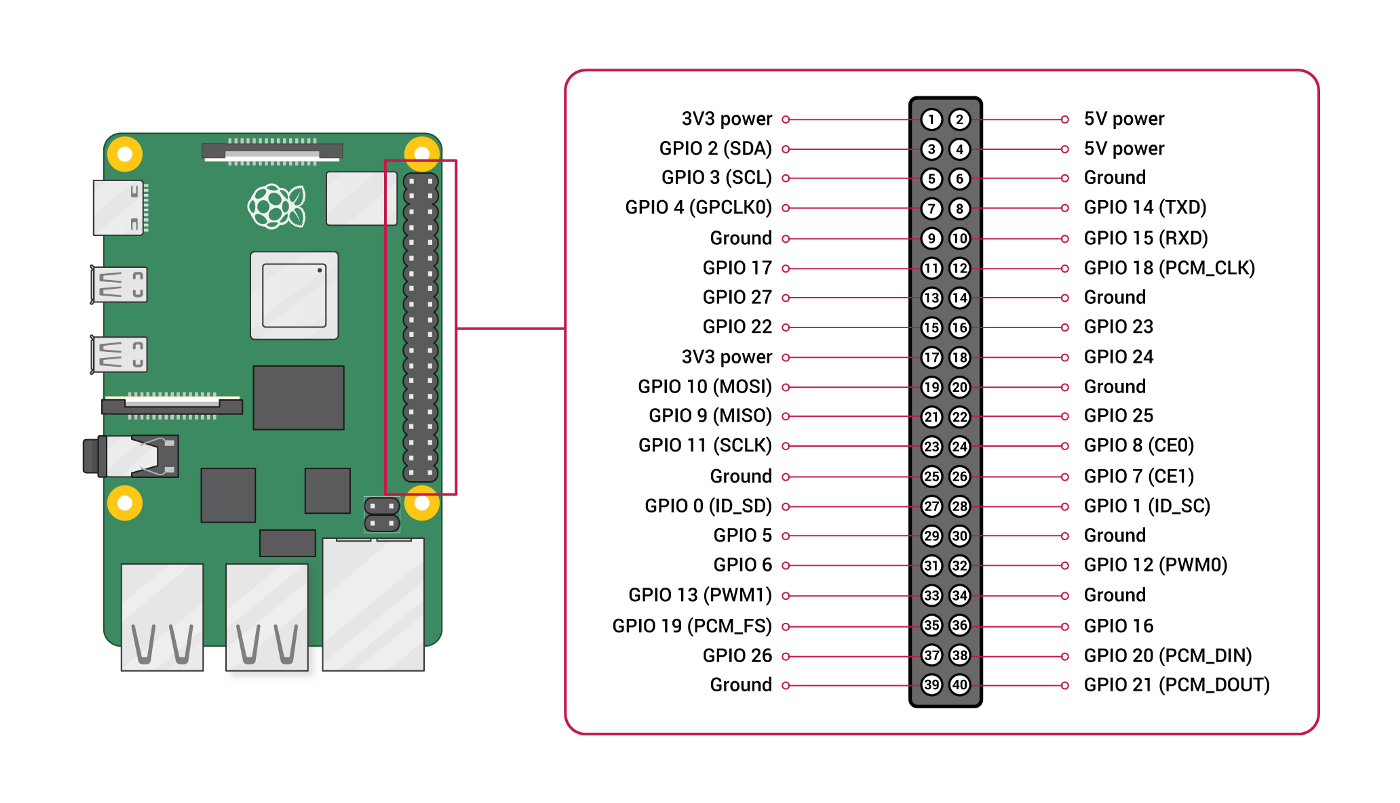
\includegraphics[scale=0.30]{Pictures/chapter05/pi_pinout.png}
\caption{Pinout van de \textit{Raspberry Pi}, bron: \url{https://www.raspberrypi.org/documentation/usage/gpio/}}
\label{fig:pi_header} % Unique label used for referencing the figure in-text
%\addcontentsline{toc}{figure}{Figure \ref{fig:webserver}} % Uncomment to add the figure to the table of contents
\end{figure}

Als het goed komen de meeste pin-fucnties bekend voor, want deze zijn vergelijkbaar met de \textit{Arduino}. Zo heeft de \textit{Pi}:
\begin{enumerate}
	\item[-] $28$ digitale \textit{GPIO}-pinnen, vergelijkbaar met de digitale pinnen op de \textit{Arduino}.
	\item[-] $2$ \textit{PWM}-pinnen, om analoge signalen mee na te bootsen.
	\item[-] Een \textit{SPI}-bus (\textit{MOSI, MISO, SCLK}).
	\item[-] Een \textit{$I^2C$}-bus (\textit{SDA, SCL}) (ook wel: \textit{TWI}-bus genoemd). 
	\item[-] Een \textit{UART} (\textit{TXD, RXD}), vergelijkbaar met de \textit{Serial} op de \textit{Arduino}.
\end{enumerate}

\begin{exercise}
Geen zin om de functie van elk pinnetje te onthouden? Open op je \textit{Pi} een \textit{Terminal}-venster en typ '\textit{pinout}'.
\end{exercise}

\newpage

\section{GPIO}\index{GPIO}
Tijd om de pinnen daadwerkelijk te gaan gebruiken. We beginnen maar eens door de \textit{GPIO}-poorten te gebruiken als output, met het aansturen van een LED.
\subsection{GPIO: output}\index{GPIO: output}
Sluit een \textit{LED} en een weerstand (van ongeveer $300 \Omega$) aan op \textit{GPIO17}. Zie ook afbeelding \ref{fig:pi_led}, hieronder:
\begin{figure}[h!]
\centering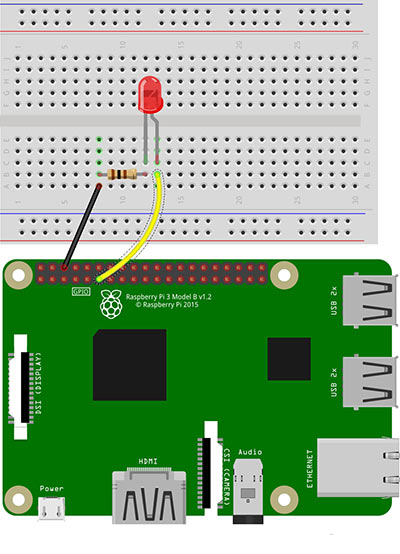
\includegraphics[scale=0.45]{Pictures/chapter05/pi_led_01.jpg}
\caption{LED aangesloten op \textit{GPIO17}}
\label{fig:pi_led} % Unique label used for referencing the figure in-text
%\addcontentsline{toc}{figure}{Figure \ref{fig:webserver}} % Uncomment to add the figure to the table of contents
\end{figure}

Zoals altijd met programmeren, kan elk probleem opgelost worden op meerdere manieren. We gaan eerst even kijken naar de 'klassieke' manier om \textit{GPIO}-poorten aan te sturen. Open je editor en voer de onderstaande code in, sla het bestand op als een \textit{*.py}-bestand.

\begin{python}
import RPi.GPIO  # Nodig voor pinnen te kunnen besturen
import time      # Nodig voor sleep()-functie

led_pin = 17     # LED zit op GPIO17.

RPi.GPIO.setmode(RPi.GPIO.BCM)         # Benader pinnen a.h.v. hun GPIO-nummer.
RPi.GPIO.setup(led_pin, RPi.GPIO.OUT)  # Set led_pin als OUPUT

while True:
    RPi.GPIO.output(led_pin, True)   # LED aan!
    time.sleep(1)                    # Wacht 1 seconde.
    RPi.GPIO.output(led_pin, False)  # LED uit!
    time.sleep(1)                    # Wacht 1 seconde.
\end{python}

\begin{remark}
Bij het runnen krijg je nu waarschijnlijk een warning. Deze is te onderdrukken door \pyth{RPi.GPIO.setwarnings(False)} toe te voegen voordat de \pyth{setmode()}-functie wordt aangeroepen op regel $6$.
\end{remark}

Het programma heeft qua opbouw veel weg van wat we gewend waren bij de \textit{Arduino}. Met de eerste twee regels (\pyth{import}) zorgen we dat we gebruik kunnen maken van de functies in de \pyth{RPi.GPIO}- en de \pyth{time}-module. Op regel $6$ en $7$ worden de module en de poort geconfigureert (dit is vergelijkbaar wat er in de \textit{void setup()} had gestaan). Daarna begint een oneindige lus, die het daadwerkelijke lampje laat knipperen (Dit had bij de \textit{Arduino} in de \textit{void loop()} gestaan). \newline

Tot zover de 'klassieke' manier, tegenwoordig zie je steeds meer dat er gebruikt wordt gemaakt van de \pyth{gpiozero}-module. En dat ziet er dan als volgt uit:
\begin{python}
import gpiozero
import time

led = gpiozero.LED(17)  # LED aangesloten op GPIO17
 
while True: 
    led.on()       # LED aan!
    time.sleep(1)  # Wacht 1 seconde.
    led.off()      # LED uit!
    time.sleep(1)  # Wacht 1 seconde
\end{python}

De \pyth{gpiozero}-module regelt alle configuratie verder voor je, wat een stuk compactere en meer leesbare code oplevert. 
\begin{remark}
\label{sec:piledobj}
Vind je het vervelend om steeds \pyth{time.sleep()} te typen? Vervang dan regel $2$ door: 
\begin{python}
from time import sleep
\end{python}
Je kunt nu gewoon \pyth{sleep()} gebruiken, zonder '\pyth{time.}' ervoor te hoeven typen. Hetzelfde principe gaat ook op voor \pyth{gpiozero.LED()}.
\end{remark}

\newpage

\subsection{GPIO: input}\index{GPIO: input}
Het eerstvolgende wat je zou willen doen met de \textit{GPIO}-pinnen is deze natuurlijk gebruiken als input. Dat kan door er een sensor aan te hangen. Let op, de \textit{Raspberry Pi} heeft in tegenstelling tot de \textit{Arduino} geen analoge ingangen, dus de sensor moet een digitaal (hoog of laag) signaal terug geven. In z'n meest basale vorm komt dit overeen met een knopje. Zie Figuur \ref{fig:pi_button}. 

\begin{figure}[h!]
\centering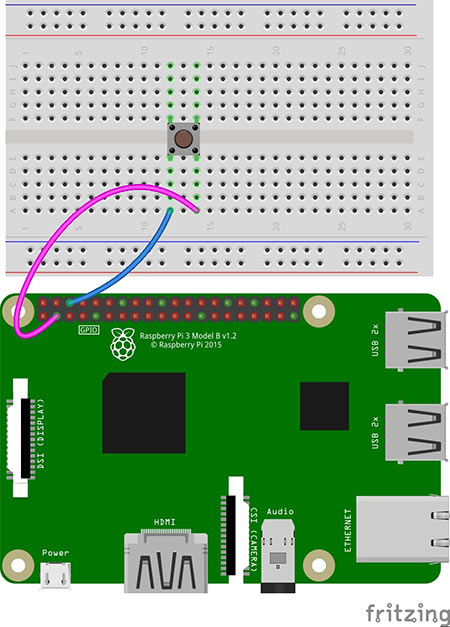
\includegraphics[scale=0.45]{Pictures/chapter05/pi_button_01.jpg}
\caption{Een drukknop aangesloten op \textit{GPIO2}}
\label{fig:pi_button} % Unique label used for referencing the figure in-text
%\addcontentsline{toc}{figure}{Figure \ref{fig:webserver}} % Uncomment to add the figure to the table of contents
\end{figure}

Ook hier gaan we eerst maar even kijken naar de 'klassieke' manier. Ook omdat dit het meest overeen komt met hoe het op de \textit{Arduino} werkt. Typ het onderstaande programma over en sla het op als een \textit{*.py} bestandd:
\begin{python}
import RPi.GPIO  # Nodig voor pinnen te kunnen besturen
from time import sleep

button_pin = 2  # Drukknop zit aangesloten op GPIO2.

# Configureer button_pin als input:
RPi.GPIO.setwarnings(False)
RPi.GPIO.setmode(RPi.GPIO.BCM)
RPi.GPIO.setup(button_pin, RPi.GPIO.IN)

while True:
    if not RPi.GPIO.input(button_pin):  # De knop is omgekeerd, vandaar 'not'.
        print('Knop ingedrukt!')
        sleep(0.25)                     # Wacht 250ms.
\end{python}

% \begin{remark}
% In plaats van de \pyth{not} in de \pyth{if}-statement zetten, zou je ook regel $9$ aan kunnen passen naar:
% \begin{python}
% RPi.GPIO.setup(button_pin, RPi.GPIO.IN, RPi.GPIO.PUD_DOWN)
% \end{python}
% Zodat er een \textit{pull-down} weerstand intern wordt gebruikt.
% \end{remark}

Zodra de knop wordt ingedrukt (we lezen de status uit door \pyth{Rpi.GPIO.input()} aan te roepen op regel $12$), wordt er iets naar het scherm geschreven dat het gelukt is.

\begin{exercise}
Wat gebeurt er als je de knop ingedrukt blijft houden? En wat als je de \pyth{sleep()} regel verwijderd?
\end{exercise}

Precies hetzelfde kunnen we ook bereiken door de \pyth{gpiozero}-module te gebruiken:
\begin{python}
from gpiozero import Button
from time import sleep 

button = Button(2)  # Drukknop zit aangesloten op GPIO2.

while True: 
    if button.is_pressed: 
        print("Knop ingedrukt!") 
        sleep(0.25)
\end{python}

Wederom een stuk compacter en to-the-point. Met deze \pyth{gpiozero}-module zijn nog veel meer mooie dingen te doen, we komen er later op terug als we leren hoe functies werken in \textit{Python}. Merk op dat we op dit moment nog steeds alles in een eindeloze \pyth{while}-loop hebben staan, dat betekend dat de \textit{Pi} enorm druk is met het draaien van ons kleine scriptje, dat kan veel efficiënter!

\newpage

\section{Huiswerkopdrachten}\index{Huiswerkopdrachten}
\begin{exercise}
Schrijf een programma waarin je met een \pyth{while}-loop de eerste $10$ getallen van de tafel van $5$ print.
\end{exercise}

\begin{exercise}
Schrijf een programma waarin je de gebruiker vraagt om een getal, en geef daarna de eerste $10$ getallen van de tafel voor dat getal. Gebruik hiervoor een \pyth{for}-loop.
\end{exercise}

\begin{exercise}
Schrijf een programma die de getallen van $-10$ t/m $-1$ op scherm print. Gebruik hiervoor alleen de \pyth{range()}-functie in de \pyth{for}-loop (en natuurlijk een \pyth{print()} ;) ).
\end{exercise}

\begin{exercise}\label{exc5:exc4}
Vraag aan de gebruiker een getal $l$, en print daarna een rij van sterretjes. Dus bij $l=7$, geeft het de volgende output:
\begin{python}
*******
\end{python}
\textbf{TIP:} Als je niet wilt dat een \pyth{print}-functie elke keer een nieuwe regel begint, kun je dit veranderen door het \textit{end}-argument te gebruiken: \pyth{print('*', end='')}. 
\end{exercise}


\begin{exercise}
Breid Vraag \ref{exc4:exc1} uit. Vraag aan de gebruiker nu $2$ getallen: $h$ en $l$. Print daarna een vierkant van sterretjes ter grootte van $h \times l$. Dus bij $h=3$ en $l=5$, geeft het de volgende output:
\begin{python}
*****
*****
*****
\end{python}
\textbf{TIP:} Je kunt loops in loops zetten. 
\end{exercise}

\begin{exercise}
Sluit een LED aan op \textit{GPIO17} en een op \textit{GPIO18}. Zorg ervoor dat de ene $1$ keer per seconde knippert en de andere $2$ keer per seconde. \newline
\textbf{TIP:} De \pyth{sleep()}-functie accepteerd ook argumenten die kleiner zijn dan $1$ (oftewel: \textit{floats}), zodat je deze ook kunt gebruiken voor delays van minder dan 1 seconde.
\end{exercise}

\begin{exercise}
Sluit een LED aan op \textit{GPIO17} en een knop op \textit{GPIO19}. Zorg ervoor dat als de knop wordt ingedrukt, de LED $10$ keer gaat knipperen. 
\end{exercise}
